\documentclass{article}
\usepackage[left=3cm,right=3cm,top=3cm,bottom=2cm]{geometry} % page settings
\usepackage{amsmath} % provides many mathematical environments & tools
\usepackage{amssymb}
\usepackage{amsfonts}
\usepackage[spanish]{babel}



\usepackage{multirow}

\usepackage{algorithm}
\usepackage{algpseudocode}
\usepackage{pifont}

\usepackage[utf8]{inputenc}
\setlength{\parindent}{0mm}

\usepackage[parfill]{parskip}

% Para el código
\usepackage{listings}
\usepackage{xcolor}
\definecolor{gray}{rgb}{0.5,0.5,0.5}
\newcommand{\n}[1]{{\color{gray}#1}}
\lstset{numbers=left,numberstyle=\small\color{gray}}

% Entorno para estilo de ejercicios
\setlength{\parindent}{0pt}

\usepackage{color}   %May be necessary if you want to color links
\usepackage{hyperref}
\hypersetup{
    colorlinks=true, %set true if you want colored links
    linktoc=all,     %set to all if you want both sections and subsections linked
    linkcolor=blue,  %choose some color if you want links to stand out
}

\usepackage{graphicx}
\usepackage{subfig}

\begin{document}

\title{%
  \huge Análisis de la eficiencia de algoritmos \\[5mm]
  \Large Algorítmica\\
  \normalsize Doble Grado en Ingeniería Informática y Matemáticas\\[5cm]
}
\author{Yábir García Benchakhtir \\ yabirgb@correo.ugr.es \\[10cm]}

\date{\today}
\maketitle

\newpage
\tableofcontents
\newpage

\section{Análisis de los algoritmos}

\section{Cálculo de la eficiencia empírica}

\subsection{Procedimiento}

Para el cálculo de la eficiencia empírica se ha automatizado el
proceso. Para ellos se han hecho 2 scripts de bash y un archivo
makefile para realizar las siguientes tareas:

\begin{itemize}
\item Crear archivos ejecutables para todos los algoritmos programados en \textit{C++} con distintas opciones de optimización a saber \textit{O1}, \textit{O2} y \textit{O3}.
\item Ejecutar los distintos tests para los intervalos programados y
  almacenar los resultados en archivos de datos.
\item Crear las respectivas gráficas para cada tabla de datos obtenida usando la herramienta gnuplot.
\end{itemize}

Para los algoritmos de medición se ha elegido un rango de datos común
en el intervalo [1000, 25000] de manera que se toman 25 medidas
haciendo incrementos de 1000 en 1000 para tomar las medidas.

$$D = \{x \in [1000, 25000]: x = 1000k, k \in \mathbb{N}\}$$

Junto a este documento se encuentran las gráficas creadas y los datos
que proporciona el programa \textit{gnuplot} sobre las mediciones.

\subsection{Condiciones de las mediciones}

Para llevar a cabo las mediciones se ha utilizado un ordenador con las siguientes características:

\begin{itemize}
\item CPU: Intel Pentium G3258 (2) @ 3.200GHz
\item Memoria RAM: 7876MiB
\item Kernel:4.13.0-36-generic
\item OS: Linux Mint 18.3 Sylvia x86\_64
\end{itemize}

A la hora de realizar los tests se ha tenido la precaución de
minimizar el uso de \textit{CPU} para no interferir en las mediciones.

\section{Análisis de los resultados}

En esta sección me he concentrado en el análisis de los resultados
obtenidos con la optimazión \textit{O0} que proporciona \textit{g++}
debido al tiempo limitado del que disponemos. Los resultados se
encuentran adjuntos para el resto de optimizaciones. Al final del
documento se hará referencia a estos datos y se usaran para
ejemplificar el efecto de la optimización.

Por simplicidad del documento los datos se recogeran en las tablas que
los comparan diferenciando claramante a que función pertenece cada
dato. Al final del documento se acompañan las medidas para las
optimizaciones de orden 1 y orden 2 para las que se han hecho medidas.

\subsection{Algoritmo de ordenación Burbuja}

Como se ha obtenido en el guión de prácticas la eficiencia de este algoritmo es:

$$ \frac{a}{2}n^2 - \frac{3a}{2}n + a \in O(n^2)$$

Observando la nuve de puntos obtenida de los resultados podemos ver
que se aproximan a una función cuadrática.

\begin{figure}[H]%
    \centering
    \subfloat[Nube de puntos]{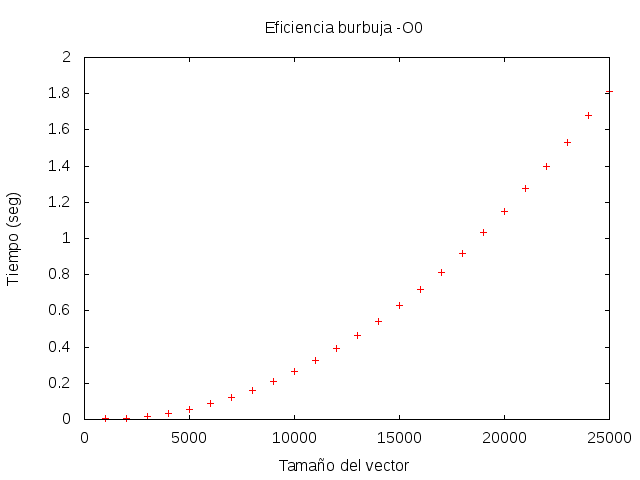
\includegraphics[width=9cm]{../plots/burbuja_O0_points.png}}%
    \qquad
    \subfloat[Función continua]{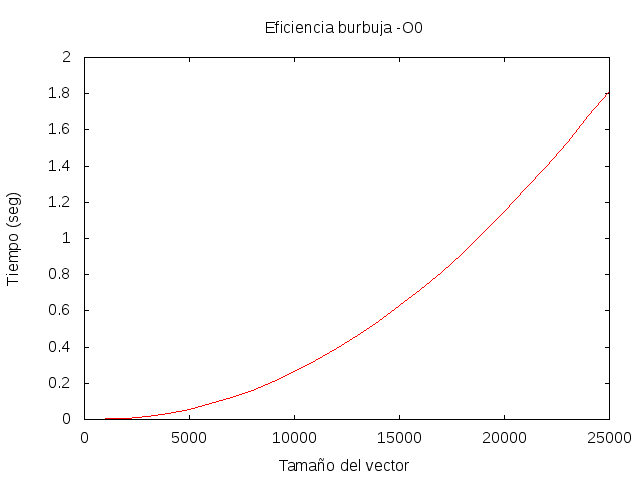
\includegraphics[width=9cm]{../plots/burbuja_O0_lines.png}}%
    \caption{Resultados experimentales representados mediante una nube de puntos y una curva continua}%
    \label{fig:example}%
  \end{figure}

Ajustando los datos por una función polinómica de orden 2, $ax^2+bx + c$, obtenemos la siguiente gráfica:

\begin{figure}[H]%
    \centering
    \subfloat{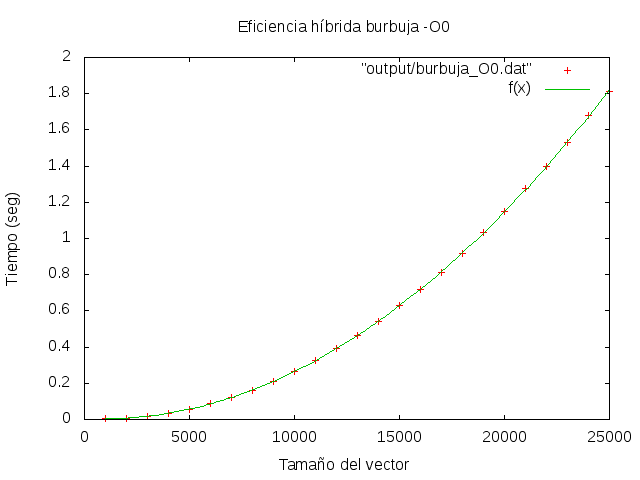
\includegraphics[width=12cm]{../plots/burbuja_O0_fit.png}}%
    \caption{Ajuste para la ordenación burbuja}%
    \label{fig:example}%
  \end{figure}

\subsection{Algoritmo de ordenación por insercción}

Observando la nuve de puntos obtenida volvemos a ver como claramente
se aproxima por una función polinómica de orden 2.

\begin{figure}[H]%
    \centering
    \subfloat[Nube de puntos]{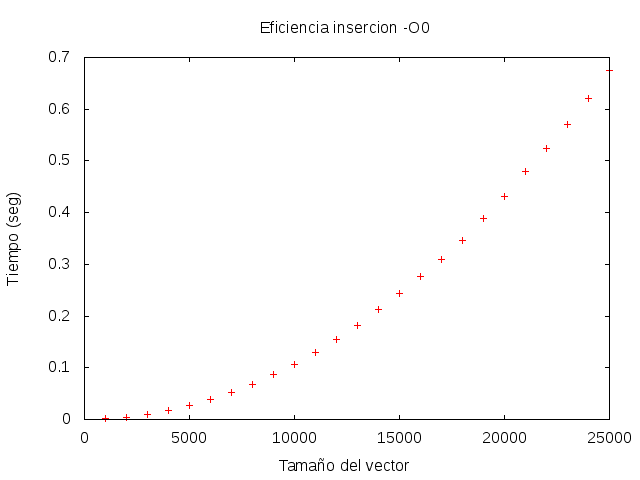
\includegraphics[width=9cm]{../plots/insercion_O0_points.png}}%
    \qquad
    \subfloat[Función continua]{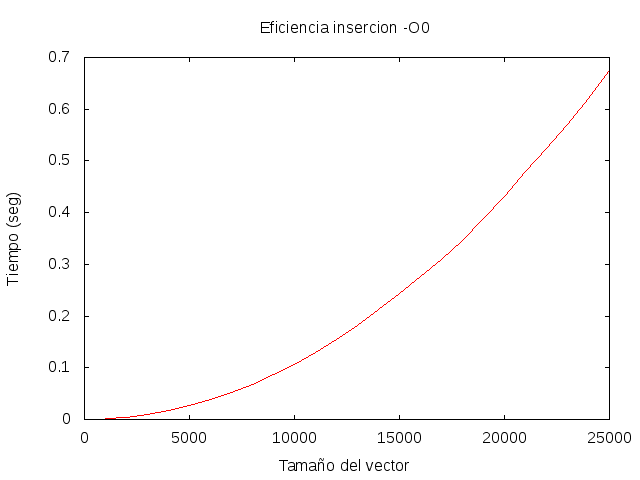
\includegraphics[width=9cm]{../plots/insercion_O0_lines.png}}%
    \caption{Resultados experimentales representados mediante una nube de puntos y una curva continua}%
    \label{fig:example}%
  \end{figure}

Ajustando los datos por una función polinómica de orden 2, $ax^2+bx + c$, obtenemos la siguiente gráfica:

\begin{figure}[H]%
    \centering
    \subfloat{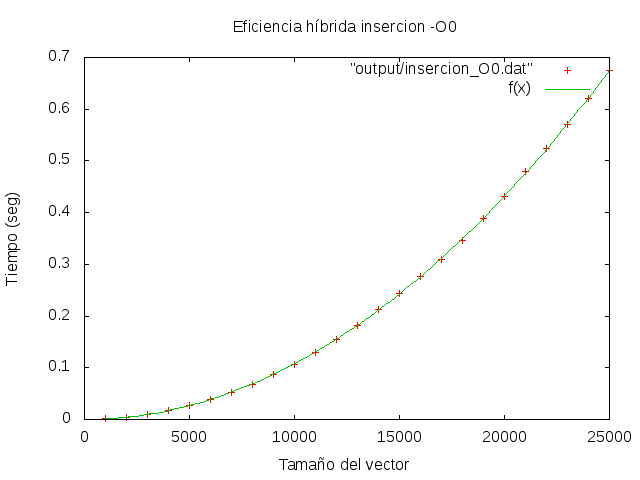
\includegraphics[width=12cm]{../plots/insercion_O0_fit.png}}%
    \caption{Ajuste para la ordenación por insercción}%
    \label{fig:example}%
\end{figure}

Comparando con la ordenación burbuja podemos ver como el tiempo que
invierte asintoticamente es mucho menor pese a ser ambas funciones de
orden cuadrático. Para ello simplemente derivamos el polinomio de
orden 2 con los coeficientes que nos ha proporcionado gnuplot tras
hacer la aproximación. En estos casos siendo $f'(x)$ la derivada para
la función de ajuste de laordenación burbuja y $g'(x)$ la derivada
para la del algoritmo por insercción obtenemos:

\begin{align}
  f'(x) & = 2\cdot 3.11435e-09x + -5.06528e-06 \\
  g'(x) & = 2\cdot1.06413e-09x + 1.06413e-09
\end{align}

\subsection{Algoritmo de ordenación por selección}

Este es el último de los algoritmos de orden cuadrático que tenemos en nuestro estudio.
  
\begin{figure}[H]%
    \centering
    \subfloat[Nube de puntos]{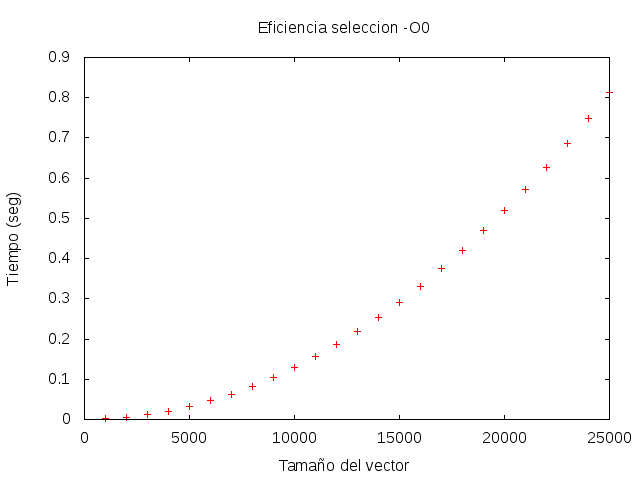
\includegraphics[width=9cm]{../plots/seleccion_O0_points.png}}%
    \qquad
    \subfloat[Función continua]{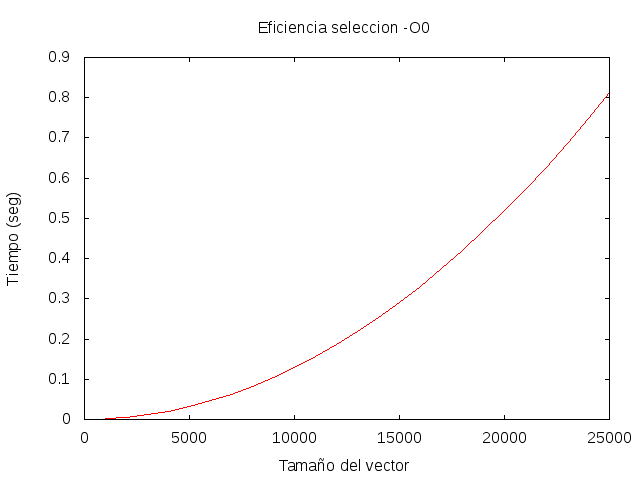
\includegraphics[width=9cm]{../plots/seleccion_O0_lines.png}}%
    \caption{Resultados experimentales representados mediante una nube de puntos y una curva continua}%
    \label{fig:example}%
\end{figure}


La nube de puntos nos permite ver que de nuevo se trata de una función
polinómica de orden 2. La gráfica de la función de ajuste es la
siguiente:

\begin{figure}[H]%
    \centering
    \subfloat{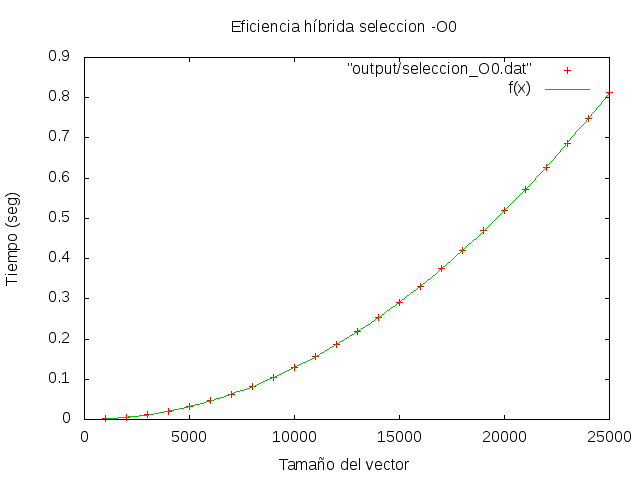
\includegraphics[width=12cm]{../plots/seleccion_O0_fit.png}}%
    \caption{Ajuste para la ordenación por selección}%
    \label{fig:example}%
\end{figure}

que aproxima visiblemente de manera muy buena a nuestros puntos.


  
\section{Comparación entre algoritmos}
Los resultados empíricos tras haber realizado las mediciones se han recogido en la siguiente tabla:
\input{tables/ordenacion.tex}

Una gráfica que nos permite visualizar estos datos es la siguiente:

\begin{figure}[H]%
    \centering
    \subfloat{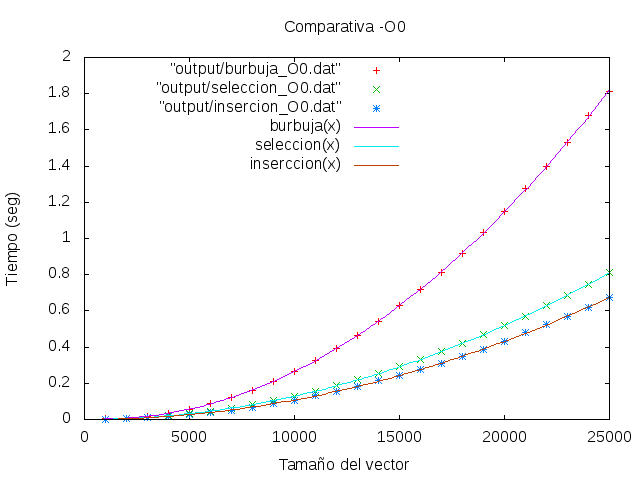
\includegraphics[width=12cm]{../plots/cuadraticas_O0.png}}%
    \caption{Comparación entre los distintos algoritmos de ordenación cuadráticos}%
    \label{fig:example}%
\end{figure}


\end{document}